%% teaser
\begin{frame}

  \frametitle{But what are \textit{droplets}?}

  \begin{columns}[T]
    %\begin{column}{0.01\textwidth} \end{column}
    
    \begin{column}{0.32\textwidth}
      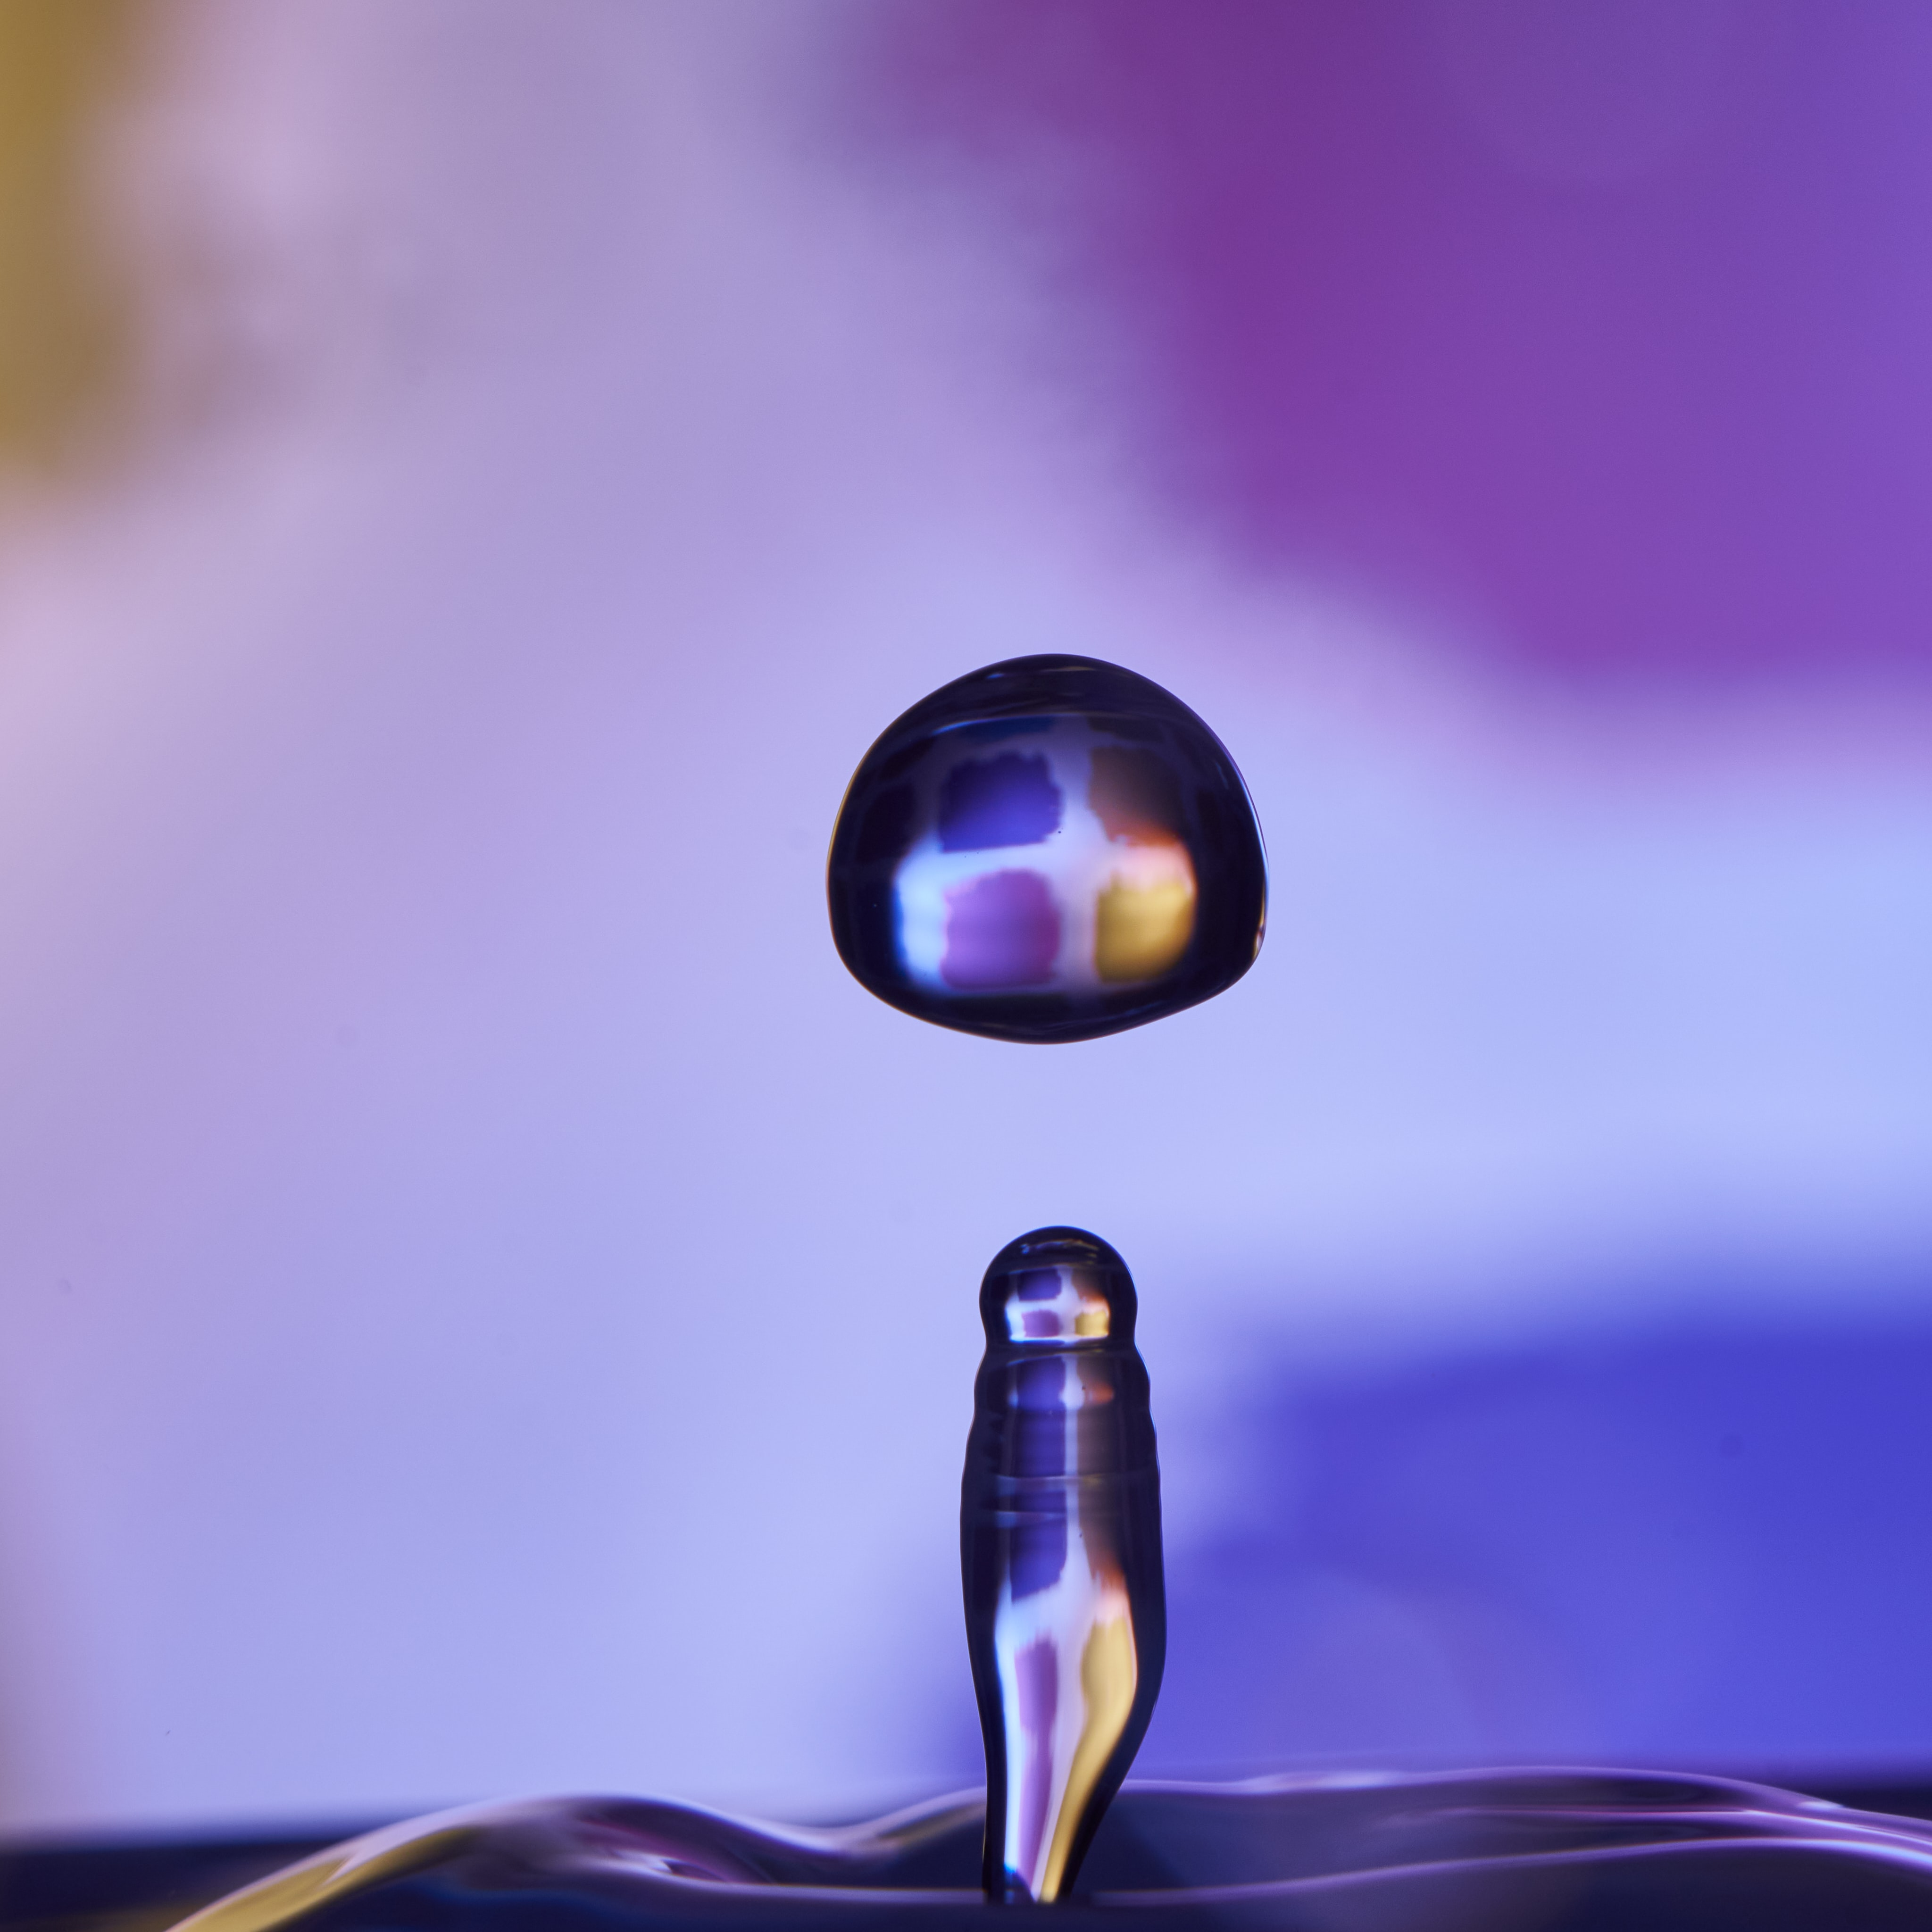
\includegraphics[height=4.8cm]{imgs/droplet_martin-brechtl-unsplash.jpg}
      \vskip.3cm
      Droplets are micron to millemetre sized liquid balls.%
      \footnote<.->[frame]{Photo by Martin Brechtl on Unsplash.}
    \end{column}

    \begin{column}{0.45\textwidth}
      \movie[showcontrols]{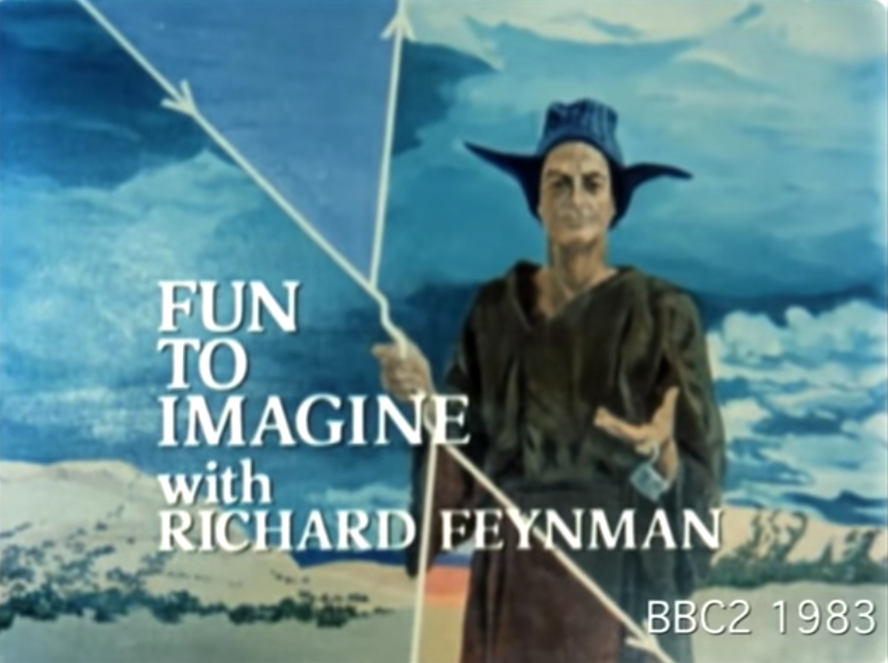
\includegraphics[height=4.8cm]{imgs/St_Feynman.png}}
            {videos/droplet_Feynman.mp4}
      \vskip.3cm
      BBC interview of Richard Feynman (1983).%
      \footnote<.->[frame]{Source: \texttt{https://youtu.be/P1ww1IXRfTA}.}
    \end{column}
  \end{columns}

  \pause
  \vskip.5cm
  \centering
  \textcolor{bb}{\bf Let's have some fun!}
  
\end{frame}

%% outline
\begin{frame}{Outline}
  \protect\hypertarget{outline}{}
  \tableofcontents
\end{frame}

%%
\hypertarget{part1}{%
  \section{Part I: Fabricating Photonic Crystals (PhC)}}

%% 
\hypertarget{background1}{%
  \subsection{Background, motivation and challenge}}

\begin{frame}
  \frametitle{Background, motivation and challenge}

  Photonic crystals (PhC) are materials patterned with a periodicity in dielectric constant
  and show great potential for building sophisticated optical circuitry that can
  route, filter, store or suppress optical signals

  \begin{figure}
    \centering
    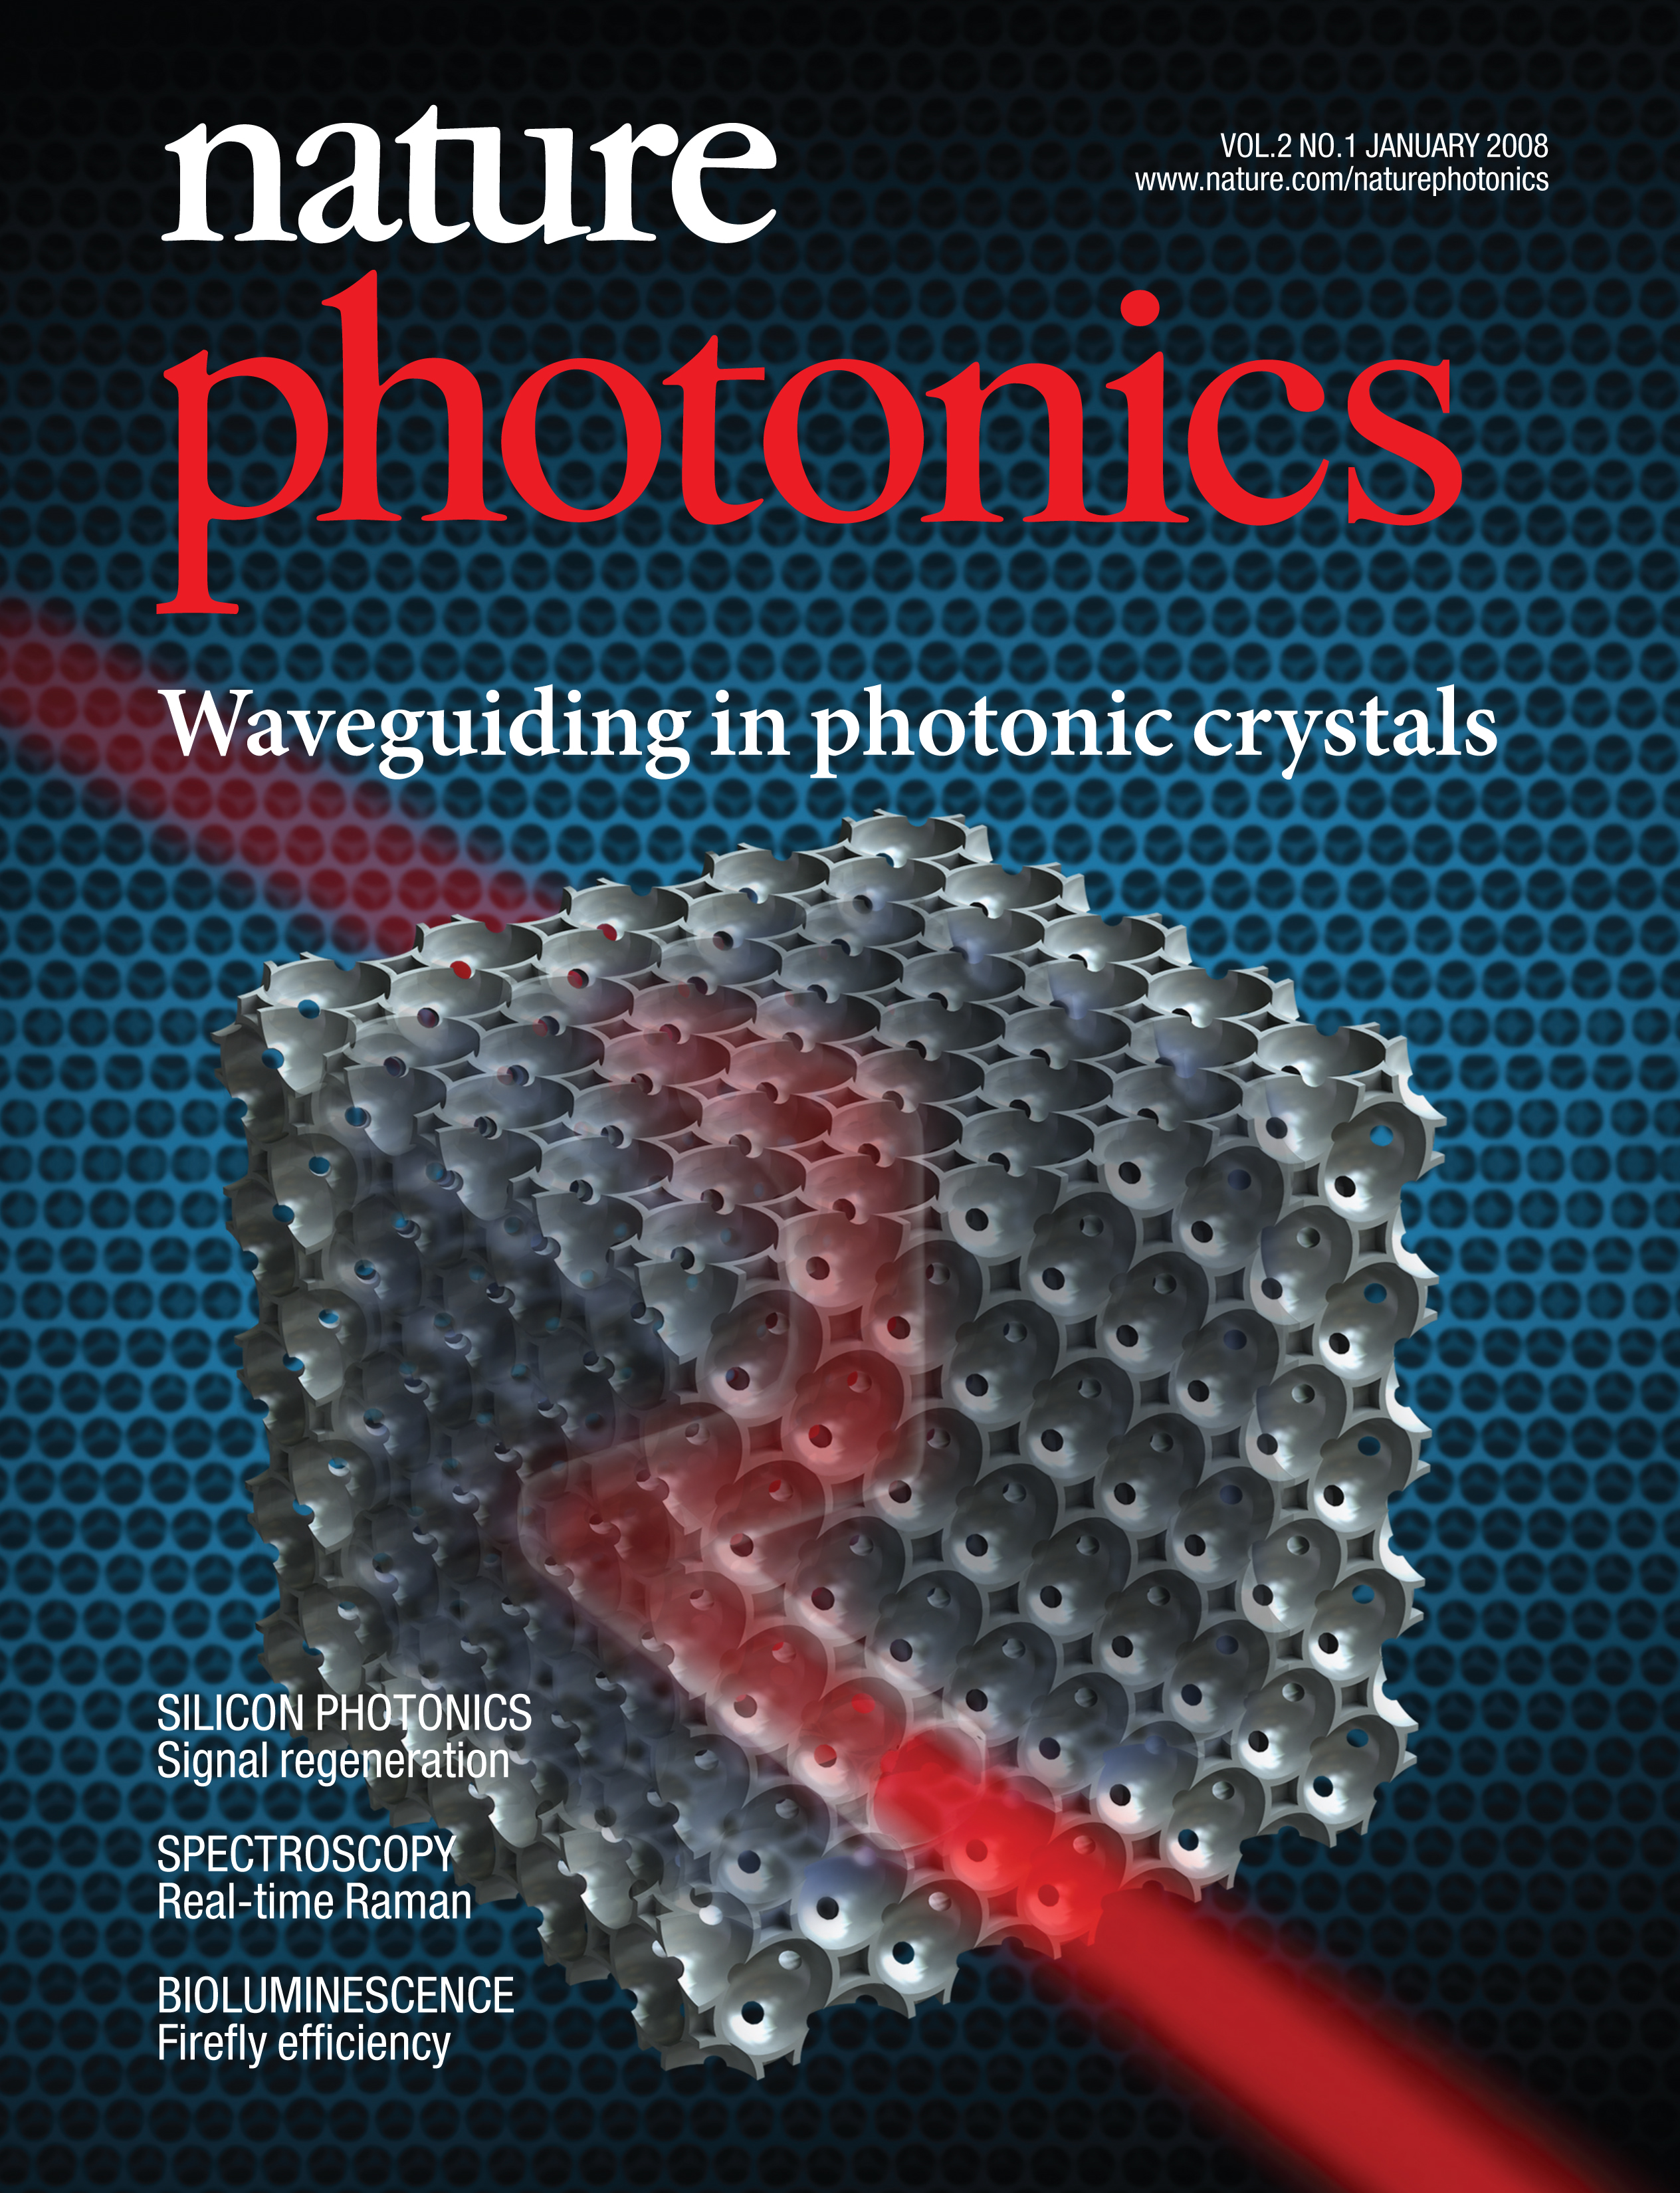
\includegraphics[height=4.73cm]{imgs/photonics_cover.jpg}
  \caption{(left) Cover photo of the January 2008 issue of Nature Photonics, showing an artistic rendering of a light beam passing through a 3D photonic crystal. \textcopyright \enspace Springer Nature. (right) Self-assembly of two to four droplets in a microfluidic chip; scale bars, 100 $\mu$m. Images courtesy of Dr.\ Bingqing Shen.}
  \label{fig:photonic-flow}
\end{figure}

\end{frame}

%%
\hypertarget{experiment}{%
  \subsection{Experiments, strategy and questions}}

\hypertarget{dipolar}{%
  \subsection{Simple physical models (q2D)}}

\hypertarget{simulation1}{%
  \subsection{3D numerical simulations}}

\hypertarget{ibm}{%
  \subsubsection{NS/IBM}}

\hypertarget{icls}{%
  \subsubsection{ICLS/GFM}}

\hypertarget{assembly}{%
  \subsection{Flow-assisted assembly}}

\hypertarget{conclusion1}{%
  \subsection{Conclusions}}


\hypertarget{part2}{%
  \section{Part II: Modelling Dense Suspensions (DS)}}

\hypertarget{background2}{%
  \subsection{Soft matter and rheology}}

\hypertarget{simulation2}{%
  \subsection{Numerical modelling}}

\hypertarget{sd}{%
  \subsubsection{SD}}

\hypertarget{hlgd}{%
  \subsubsection{HLGD}}

\hypertarget{conclusion2}{%
  \subsection{Outlook}}

\hypertarget{summary}{%
  \section{Summary}}

\hypertarget{acknowledgements}{%
  \section{Acknowledgements}}










\iffalse

\begin{frame}
  \frametitle{}

  In Batchelor we believe.

\end{frame}

\fi

%\begin{frame}{Background}
%\begin{columns}[T]
%\begin{column}{0.5\textwidth}
%\textbf{Atmospheric energy
%spectrum}%\footnote<.->[frame]{\citet{NastromGage1985} © AMS}
%
%%\includegraphics[width=\textwidth,height=0.9\textheight]{../imgs/NastromGage.png}
%\end{column}
%
%\begin{column}{0.5\textwidth}
%\pause
%
%Two inertial ranges, separated by scales:
%
%~
%
%\begin{itemize}
%\tightlist
%\item
%  planetary / synoptic scales \(E(k) \sim k^{-3}\)
%  %\includegraphics[width=0.7\textwidth,height=0.28\textheight]{../imgs/synoptic.jpg}
%\end{itemize}
%
%\pause
%
%\begin{itemize}
%\tightlist
%\item
%  mesoscales \(E(k) \sim k^{-5/3}\)
%  %\includegraphics[width=0.7\textwidth,height=0.28\textheight]{../imgs/mesoscale.jpg}
%\end{itemize}
%\end{column}
%\end{columns}
%
%\pause
%
%\centering{\alert{How do we theorize the mechanism behind these two inertial ranges?}}
%\end{frame}
%%
%%\begin{frame}{Two-dimensional turbulence}
%%\protect\hypertarget{two-dimensional-turbulence}{}
%%Kraichnan's theory of 2D
%%turbulence\footnote<.->[frame]{\citet{Kraichnan1967}}
%%
%%\begin{itemize}
%%\item
%%  \textbf{Vorticity} and \textbf{enstrophy} conservation: a strong
%%  constraint on cascade
%%\item
%%  Dual cascade:
%%  \[E(k) \sim \epsilon^{2/3}k^{-5/3},\quad E(k) \sim \eta^{2/3}k^{-3}\]
%%\end{itemize}
%%
%%\pause
%%
%%\begin{itemize}
%%\item
%%  Directions of cascades:
%%
%%  \begin{itemize}
%%  \item
%%    \(k^{-5/3}\) range: constant energy
%%    flux\footnote<.->[frame]{Similar to scaling due to \citet{Kolmogorov1941}, \citet{obukhov1941distribution} and \citet{obukhov1941spectral}}
%%    \(\epsilon\), \textbf{inverse} cascade
%%  \item
%%    \(k^{-3}\) range: constant enstrophy flux \(\eta\), \textbf{forward}
%%    cascade
%%  \end{itemize}
%%\end{itemize}
%%
%%\pause
%%
%%\begin{itemize}
%%\tightlist
%%\item
%%  Spatial scales of inertial ranges: ``a
%%  paradox''\footnote<.->[frame]{\citet{Frisch}}
%%  \includegraphics[width=\textwidth,height=0.5\textheight]{../imgs/cascade_horiz.png}
%%\end{itemize}
%%\end{frame}
%%
%%\begin{frame}{Possible explanations of mesoscale spectrum}
%%\protect\hypertarget{possible-explanations-of-mesoscale-spectrum}{}
%%\begin{bluecolorbox}[Hypotheses for cascade
%%directions]\label{hypotheses-for-cascade-directions}
%%
%%\begin{itemize}
%%\item
%%  \citet{Gage:1979} \& \citet{Lilly:1983}: \textbf{inverse energy
%%  cascade} as in \citet{Kraichnan1967}
%%\item
%%  \citet{Dewan:1979}: \textbf{forward energy cascade} as in
%%  \citet{Kolmogorov1941}
%%\end{itemize}
%%
%%\end{bluecolorbox}
%%
%%\pause
%%
%%\begin{bluecolorbox}[Vertical resolutions]\label{vertical-resolutions}
%%
%%\begin{itemize}
%%\tightlist
%%\item
%%  \citet{Waite-Bartello:2004} and \citet{Lindborg2006} :
%%  \textbf{stratified turbulence}. \(l_v \sim u/N \approx 1 \text{km}\).
%%\item
%%  \citet{Callies-Buhler-Ferrari:2016} : \textbf{inertia gravity waves}.
%%  Frequency \(\omega \approx f\). i.e.~\(l_v \approx\) 100 metres.
%%\end{itemize}
%%
%%\end{bluecolorbox}
%%
%%\pause
%%
%%~
%%
%%\begin{columns}[T]
%%\begin{column}{0.4\textwidth}
%%DNS of stratified turbulence supports:
%%\footnote<.->[frame]{\citet{Lindborg2006} }
%%
%%\begin{itemize}
%%\item
%%  \(k^{-5/3}\) spectrum
%%\item
%%  \textbf{forward cascade}
%%\item
%%  \textbf{fine vertical resolution} requirement
%%\end{itemize}
%%\end{column}
%%
%%\begin{column}{0.48\textwidth}
%%\pause
%%
%%General circulation
%%models\footnote<.->[frame]{\citet{Augier-Lindborg:2013}} shows:
%%
%%\begin{itemize}
%%\item
%%  \(k^{-5/3}\) spectrum
%%\item
%%  \textbf{forward cascade} in mesoscales
%%\item
%%  with \textbf{coarse resolution}: 24 pressure levels along vertical
%%\end{itemize}
%%\end{column}
%%\end{columns}
%%
%%\pause
%%
%%\vspace{20pt}
%%
%%\centering{{\alert{Minimum number of vertical levels? Is it possible with a single level model?}}}
%%\end{frame}
%%
%%\begin{frame}{Quasi geostrophic equation}
%%\protect\hypertarget{quasi-geostrophic-equation}{}
%%Quasi-geostrophic equation\footnote<.->[frame]{\citet{Charney1971}}
%%conserves an approximate \emph{potential vorticity}: \[\Dt{q} = 0,\]
%%\[ q = \nabla^2 \psi + \frac{\alert<2>{f_0}^2}{\tilde \rho}
%%  \left(\frac{\tilde \rho}{\alert<3>{N^2}} \alert<3>{\p_z \psi} \right) + \alert<2>{\beta} y, \]
%%
%%\pause
%%
%%\begin{itemize}
%%\item
%%  Incorporates {\alert<2>{rotation}} and {\alert<3>{stratification}} in
%%  a 2D model
%%\item
%%  \onslide<4->{Bridging \textbf{ideal 2D turbulence} to
%%  \textbf{atmospheric turbulence}}
%%\item
%%  \onslide<5->{Valid for \textbf{strong rotation}, lengths scales
%%  \textbf{smaller than planetary} scales}
%%\item
%%  \onslide<6->{No ageostrophic motion, for example: \textbf{inertial
%%  gravity waves}}
%%\item
%%  \onslide<7->{Reproduces \(k^{-3}\) spectrum}
%%\end{itemize}
%%
%%~
%%
%%\onslide<7->{\centering{{\alert{What about the $k^{-5/3}$ mesoscale spectrum?}}}}
%%\end{frame}
%%
%%\hypertarget{shallow-water-equations}{%
%%\subsection{Shallow water equations}\label{shallow-water-equations}}
%%
%%\begin{frame}{Properties of shallow water equations}
%%\protect\hypertarget{properties-of-shallow-water-equations}{}
%%\begin{block}{Governing equations}
%%\protect\hypertarget{governing-equations}{}
%%\note{\begin{itemize}
%%\tightlist
%%\item
%%  Inviscid equations conserves in a periodic domain (no boundary fluxes)
%%\end{itemize}}
%%
%%\begin{columns}[T]
%%\begin{column}{0.5\textwidth}
%%\begin{align*}
%%  \partial_t \alert<2>{\mathbf{u}} &= - (\alert<2>{\mathbf{u}}.\nabla) \alert<2>{\mathbf{u}}
%%      - \alert<3>c^2 \nabla \alert<5>h - \alert<4>f\mathbf{e_z} \times \alert<2>{\mathbf{u}}, \\
%%  \partial_t \alert<5>h &= - \nabla \cdot (\alert<5>h \alert<2>{\mathbf{u}}).
%%  \end{align*}
%%
%%\begin{itemize}
%%\item
%%  where,
%%
%%  \begin{itemize}
%%  \tightlist
%%  \item
%%    \onslide<2->{\(\alert<2>{\mathbf{u}}=\) horizontal velocity vector,}
%%  \item
%%    \onslide<3->{\(\alert<3>{c} =\) wave speed,}
%%  \item
%%    \onslide<4->{\(\alert<4>f\) = Coriolis parameter,}
%%  \item
%%    \onslide<5->{\(\alert<5>{h} = 1 + \eta\), non-dimensional height of
%%    fluid\footnote<.->[frame]{\citet{vallis_atmospheric_2017}}.}
%%  \end{itemize}
%%\end{itemize}
%%\end{column}
%%
%%\begin{column}{0.5\textwidth}
%%\onslide<5->{\includegraphics[width=1\textwidth,height=0.4\textheight]{../imgs/swe_eta_h.png}}
%%\end{column}
%%\end{columns}
%%
%%\onslide<6->
%%
%%\begin{greencolorbox}[with \textbf{good
%%properties}]\label{with-good-properties}
%%
%%\begin{itemize}
%%\tightlist
%%\item
%%  Conserves \textbf{energy} \(E = E_K + E_P\) and the sum \(E_K + E_A\),
%%  where \(E_A =\) available potential energy (A.P.E.)
%%\item
%%  Conserves \textbf{potential vorticity}, \(Q = (\zeta + f)/h\)
%%\item
%%  Equipartition of \(E_K\) and \(E_A\) over a wave period
%%\end{itemize}
%%
%%\end{greencolorbox}
%%
%%\onslide<7->
%%
%%\begin{redcolorbox}[and some
%%\textbf{downsides}]\label{and-some-downsides}
%%
%%\begin{itemize}
%%\tightlist
%%\item
%%  Waves \(\to\) shocks
%%\item
%%  Cubic \(E_K = h\mathbf{u.u} / 2\)
%%\end{itemize}
%%
%%\end{redcolorbox}
%%\end{block}
%%\end{frame}
%%
%%\begin{frame}{Results: Energy
%%cascade\footnote<.->[frame]{ \citet{augier_shallow_2019} }}
%%\protect\hypertarget{results-energy-cascade}{}
%%\begin{bluecolorbox}[SW analogue of \citet{Kolmogorov1941}'s
%%\(\frac{4}{5}\) law for \(3^{rd}\)-order structure
%%function]\label{sw-analogue-of-kolmogorov1941s-frac45-law-for-3rd-order-structure-function}
%%
%%\begin{equation*}
%%  \meane{ |\delta \uu|^2 \delta J_L }
%%  + c^2\meane{ (\delta h)^2 \delta u_L } = -4 \epsilon r,
%%  \end{equation*}
%%
%%\begin{itemize}
%%\tightlist
%%\item
%%  \(\epsilon =\) energy flux or dissipation; \(r =\) separation distance
%%\item
%%  \(J_L \equiv h u_L\) and \(u_L \equiv \uu\cdot\rr / |\rr|\) are
%%  longitudinal momentum and velocities
%%\item
%%  positive flux (\(\epsilon > 0\)) \(\Rightarrow\) \textbf{forward
%%  energy} cascade
%%\end{itemize}
%%
%%\end{bluecolorbox}
%%
%%\pause
%%
%%\begin{figure}
%%\centering
%%\includegraphics[width=\textwidth,height=0.5\textheight]{../paper_04_shallow_water/Pyfig/fig3-eps-converted-to.pdf}
%%\caption{Spectral energy fluxes \(\Pi(k)\) and \(3^{rd}\)-order
%%structure functions \(\approx-4\epsilon r\)}
%%\end{figure}
%%\end{frame}
%%
%%\begin{frame}{Results: Shock
%%waves\footnote<.->[frame]{ \citet{augier_shallow_2019} }}
%%\protect\hypertarget{results-shock-waves}{}
%%\begin{columns}[T]
%%\begin{column}{0.65\textwidth}
%%\begin{figure}
%%\centering
%%\includegraphics[width=\textwidth,height=0.8\textheight]{../paper_04_shallow_water/Pyfig/fig5-eps-converted-to.pdf}
%%\caption{Visualization of shocks using divergence \(\nabla.\uu\) and
%%velocity component \(u_y\)}
%%\end{figure}
%%\end{column}
%%
%%\begin{column}{0.48\textwidth}
%%\begin{block}{Highlights}
%%\protect\hypertarget{highlights}{}
%%\begin{itemize}
%%\item
%%  Parameters
%%
%%  \begin{itemize}
%%  \tightlist
%%  \item
%%    Top: \(n=1920\), \(c=20\)
%%  \item
%%    Bottom: \(n=1920\), \(c=400\)
%%  \end{itemize}
%%\item
%%  \(F_f \propto 1 / c\)
%%\item
%%  \(\nabla. \uu < 0 \Rightarrow\) shock
%%\end{itemize}
%%\end{block}
%%\end{column}
%%\end{columns}
%%\end{frame}
%%
%%\begin{frame}{Results: Spectra and higher-order
%%statistics\footnote<.->[frame]{ \citet{augier_shallow_2019} }}
%%\protect\hypertarget{results-spectra-and-higher-order-statistics}{}
%%\begin{bluecolorbox}[Scaling laws for shock dominated
%%turbulence]\label{scaling-laws-for-shock-dominated-turbulence}
%%
%%\begin{itemize}
%%\item
%%  \onslide<+->{Shock amplitudes,
%%  \(| \Delta u | \sim | c \Delta h | \sim (\epsilon d)^{1/3}\)}
%%\item
%%  \onslide<+->{\(p^{th}\)-order structure functions
%%  \[\meane{|\delta u |^p}  \sim \meane{(c|\delta h |)^p} \sim  (\epsilon
%%  d)^{p/3} \,  \frac{r}{d}\]}
%%\item
%%  \onslide<+->{\(p = 2 \Rightarrow\) energy spectra:
%%  \(E_K(k) \sim E_A(k) \sim \epsilon ^{2/3} d^{-1/3} k^{-2}\)}
%%\end{itemize}
%%
%%\end{bluecolorbox}
%%
%%\pause
%%
%%\vspace{-10pt}
%%
%%\begin{figure}
%%\centering
%%
%%\subfloat[\(d/L_f \sim F_f^{1/2}\)]{\includegraphics[width=\textwidth,height=0.44\textheight]{../paper_04_shallow_water/Pyfig/fig6.eps}\label{fig:D}}
%%\subfloat[\(E(k) \sim k ^{-2}\)]{\includegraphics[width=\textwidth,height=0.44\textheight]{../paper_04_shallow_water/Pyfig/fig10.eps}\label{fig:E}}
%%
%%\caption{Shock separation \(d\) and energy spectra \(E(k)\) scaling}
%%
%%\label{fig:scaling}
%%
%%\end{figure}
%%\end{frame}
%%
%%\hypertarget{toy-model-equations}{%
%%\subsection{Toy model equations}\label{toy-model-equations}}
%%
%%\begin{frame}{Derivation of toy model
%%equations\footnote<.->[frame]{\citet{LindborgMohanan2017}}}
%%\protect\hypertarget{derivation-of-toy-model-equations}{}
%%\note{with \(\Psi\) and \(\chi\) being the \textbf{stream function} and
%%the \textbf{velocity potential} respectively.}
%%
%%\begin{block}{Helmholtz decomposition}
%%\protect\hypertarget{helmholtz-decomposition}{}
%%\[{\bf u} = \bf{u}_r + \bf{u}_d\]
%%
%%\begin{itemize}
%%\tightlist
%%\item
%%  \({\bf u}_r = -\nabla \times ( {\bf e_z} \Psi)\) is the rotational
%%  component
%%\item
%%  \(\bf {u}_d = \nabla \chi\) is the divergent component
%%\end{itemize}
%%
%%\pause
%%\end{block}
%%
%%\begin{block}{Governing equations}
%%\protect\hypertarget{governing-equations-1}{}
%%\begin{itemize}
%%\tightlist
%%\item
%%  Starting from classical shallow water equations,
%%\end{itemize}
%%
%%\begin{bluecolorbox}[Assumptions \&
%%modifications]\label{assumptions-modifications}
%%
%%\begin{itemize}
%%\item
%%  \onslide<2->{{\alert<2>{\textbf{Surface displacement much smaller}}}
%%  compared to the mean fluid layer height, \(\eta << 1\).}
%%\item
%%  \onslide<4->{Velocities in the large scale are
%%  {\alert<4>{\textbf{dominated by rotational part}}},
%%  \(|\bf u_r| >> |\bf u_d|\).}
%%\item
%%  \onslide<6->{{\alert<6>{\textbf{Substitute}}} \(c\eta\) with
%%  \(\theta\) (optional).}
%%\end{itemize}
%%
%%\end{bluecolorbox}
%%
%%\begin{align*}
%%\frac{\partial {\bf u}} {\partial t} + {
%%  \color<4>{purple}\only<-4>{{\uu}\, \cdot\, \nabla}
%%  \color<5->{teal}\only<5->{{\uu_r}\cdot \nabla}
%%  }
%%  {\bf u} +
%%  f {\bf e}_z \times {\bf u} &=
%%  \color<6>{purple}\only<-6>{-c^2 \nabla \eta} %
%%  \color<7->{teal}\only<7->{-c \nabla \theta} %
%%  \\
%%\frac{\partial 
%%  \color<6>{purple}\only<-6>\eta
%%  \color<7->{teal}\only<7->\theta
%%}{\partial t}+ {
%%  \color<4>{purple}\only<-4>{{\uu}\, \cdot\, \nabla}
%%  \color<5->{teal}\only<5->{{\uu_r}\cdot \nabla}
%%  }
%%  \color<6>{purple}\only<-6>\eta
%%  \color<7->{teal}\only<7->\theta
%%  &= -
%%  \color<7->{teal}\only<7->c
%%  \color<2>{purple}\only<2>{(1+\eta) \nabla \cdot {\bf u}}
%%  \color<3->{teal}\only<3->{\nabla \cdot {\bf u}}
%%\end{align*}
%%
%%\begin{itemize}
%%\tightlist
%%\item
%%  \onslide<7->{\color{teal}{Q.E.D.}}
%%\end{itemize}
%%\end{block}
%%\end{frame}
%%
%%\begin{frame}{A good
%%compromise\footnote<.->[frame]{\citet{LindborgMohanan2017}}}
%%\protect\hypertarget{a-good-compromise}{}
%%\begin{greencolorbox}[Pros]\label{pros}
%%
%%\begin{itemize}
%%\item
%%  \textbf{No shocks}
%%\item
%%  Kinetic and available potential energies are \textbf{quadratic} and
%%  conserved
%%\item
%%  \textbf{Linearised potential vorticity} \(q\) conserved in the limit
%%  of strong rotation \(Ro \to 0\), where \(q=\zeta - f \eta\)
%%\end{itemize}
%%
%%\end{greencolorbox}
%%
%%\begin{redcolorbox}[Cons]\label{cons}
%%
%%\begin{itemize}
%%\tightlist
%%\item
%%  \textbf{Full potential vorticity} \(Q\) is not exactly conserved
%%\end{itemize}
%%
%%\end{redcolorbox}
%%
%%\begin{columns}[T]
%%\begin{column}{0.58\textwidth}
%%\centering{%
%%  {%
%%  \movie[
%%    width=8.5cm,
%%    height=4.3cm,
%%    showcontrols,
%%    poster,
%%    autostart, loop
%%  ]{}{./videos/toy_model_qa.mp4}
%%
%%  Video: Time lapse of potential vorticity ($q$) & wave field}
%%}
%%\end{column}
%%
%%\begin{column}{0.48\textwidth}
%%\begin{figure}
%%\centering
%%\includegraphics[width=\textwidth,height=4.3cm]{../paper_03_toy_model/fig13.eps}
%%\caption{Blown-up view of a strong anticyclonic vortex \& the wave
%%field}
%%\end{figure}
%%\end{column}
%%\end{columns}
%%\end{frame}
%%
%%\begin{frame}{Energy spectra}
%%\protect\hypertarget{energy-spectra}{}
%%\begin{columns}[T]
%%\begin{column}{0.65\textwidth}
%%\begin{figure}
%%\centering
%%
%%\subfloat[\(k_f = 6\delta k\)]{\includegraphics[width=\textwidth,height=0.75\textheight]{../paper_03_toy_model/fig3.eps}\label{fig:speck6}}
%%\subfloat[\(k_f = 30\delta k\)]{\includegraphics[width=\textwidth,height=0.75\textheight]{../paper_03_toy_model/fig11.eps}\label{fig:speck30}}
%%
%%\caption{Time averaged energy spectra from two simulations by forcing at
%%different forcing wavenumbers (\(k_f\))}
%%
%%\label{fig:spectratoy}
%%
%%\end{figure}
%%\end{column}
%%
%%\begin{column}{0.48\textwidth}
%%\begin{block}{Highlights}
%%\protect\hypertarget{highlights-1}{}
%%\begin{itemize}
%%\tightlist
%%\item
%%  Legend
%%
%%  \begin{itemize}
%%  \tightlist
%%  \item
%%    \(E_K =\) {\color{red}{kinetic energy}}
%%  \item
%%    \(E_A =\) {\color{blue}{available potential energy}}
%%  \item
%%    \(E_W =\) {\color{violet}{wave energy}}
%%  \item
%%    \(E_V =\) {\color{teal}{vortical energy}}
%%  \end{itemize}
%%\item
%%  \(E_W \sim k^{-5/3}\)
%%\item
%%  \(E_V \sim k^{-3}\)
%%\item
%%  Equipartition between \(E_K\) and \(E_A\)
%%\end{itemize}
%%\end{block}
%%\end{column}
%%\end{columns}
%%\end{frame}
%%
%%\begin{frame}
%%\note{The total spectral energy flux \(\Pi\) has been decomposed into
%%kinetic (\(\Pi_K\)) and available potential energy (\(\Pi_A\)) energy
%%fluxes. The conversion from available potential energy to kinetic energy
%%is represented by \(C_{cum}\). The kinetic energy flux is further
%%decomposed as \(\Pi_{2D}\), the flux due to geostrophic modes and the
%%difference \(\Pi_K - \Pi_{2D}\).}
%%
%%\begin{columns}[T]
%%\begin{column}{0.55\textwidth}
%%\begin{block}{Spectral energy budget}
%%\protect\hypertarget{spectral-energy-budget}{}
%%\begin{itemize}
%%\tightlist
%%\item
%%  \textbf{Spectral energy flux},
%%  \(\Pi(\mathbf{k},t) = \int_\mathbf{k}^{\infty} T(\mathbf{k}',t) d\mathbf{k}'\)
%%\end{itemize}
%%
%%\pause
%%
%%\begin{itemize}
%%\tightlist
%%\item
%%  \(T=T_K + T_A\) are \textbf{transfer functions}, \begin{align*}
%%  \partial_t E_K(\mathbf{k},t) 
%%    &= \text{\textonehalf} \partial_t (\hat{\uu}\hat{\uu}^*)
%%    = T_K + C_K
%%    ,\quad\\
%%  \partial_t E_A(\mathbf{k},t) 
%%    &= \text{\textonehalf} \partial_t (\hat{\theta}\hat {\theta}^*)
%%    = T_A + C_A 
%%  \end{align*} which for the toy model equations are derived as
%%  \(T_K= \Im\left[\hat{u}_i^* k_j \widehat{u^r_j u_i}\right],\quad T_A = \Im\left[\hat{\theta}^* k_j \widehat{u^r_j \theta}\right]\).
%%\end{itemize}
%%\end{block}
%%\end{column}
%%
%%\begin{column}{0.48\textwidth}
%%\pause
%%
%%\begin{block}{Normal mode decomposition}
%%\protect\hypertarget{normal-mode-decomposition}{}
%%\begin{itemize}
%%\tightlist
%%\item
%%  Linearization and diagonalization of the toy model equations yields
%%  the \textbf{normal modes}: \begin{align*}
%%      \mathbf{B}
%%      = & \frac{1}{\sqrt{2}\sigma}
%%      \begin{Bmatrix} \sqrt{2} c\left(-
%%          \kappa^{2} \hat \psi +  f\hat\eta \right)               \\
%%          \kappa \left(c^{2} \eta + f \hat{\psi} + i \hat{\chi} \sigma\right) \\
%%          \kappa \left(c^{2} \eta + f \hat{\psi} - i \hat{\chi} \sigma\right)
%%      \end{Bmatrix}
%%      \propto
%%      \begin{Bmatrix}
%%          q \\
%%          a^+ \\
%%          a^-
%%      \end{Bmatrix}
%%  \end{align*} which can be transformed to
%%  \(\mathbf{U} = \{\hat{u}_x,\hat{u}_y, \hat{\theta}\}^T\).
%%\end{itemize}
%%\end{block}
%%\end{column}
%%\end{columns}
%%
%%\pause
%%
%%\begin{columns}[T]
%%\begin{column}{0.75\textwidth}
%%\begin{figure}
%%\centering
%%\includegraphics[width=\textwidth,height=0.52\textheight]{../paper_03_toy_model/fig5.eps}
%%\caption{Spectral energy fluxes from two runs with different forcing
%%schemes}
%%\end{figure}
%%\end{column}
%%
%%\begin{column}{0.48\textwidth}
%%\vspace{40pt}
%%
%%\begin{block}{Highlights}
%%\protect\hypertarget{highlights-2}{}
%%\begin{itemize}
%%\item
%%  Forcing scheme differences:
%%
%%  \begin{itemize}
%%  \tightlist
%%  \item
%%    Left: waves
%%  \item
%%    Right: vortices \& wave
%%  \end{itemize}
%%\item
%%  \(V:\) vortical mode
%%\item
%%  \(W:\) wave mode
%%\end{itemize}
%%\end{block}
%%\end{column}
%%\end{columns}
%%\end{frame}
%%
%%\begin{frame}{Comparison of a
%%GCM\footnote<.->[frame]{\citet{Augier-Lindborg:2013}} with the toy
%%model\footnote<.->[frame]{\citet{LindborgMohanan2017}}}
%%\protect\hypertarget{comparison-of-a-gcm-with-the-toy-model}{}
%%\begin{figure}
%%\centering
%%
%%\subfloat[]{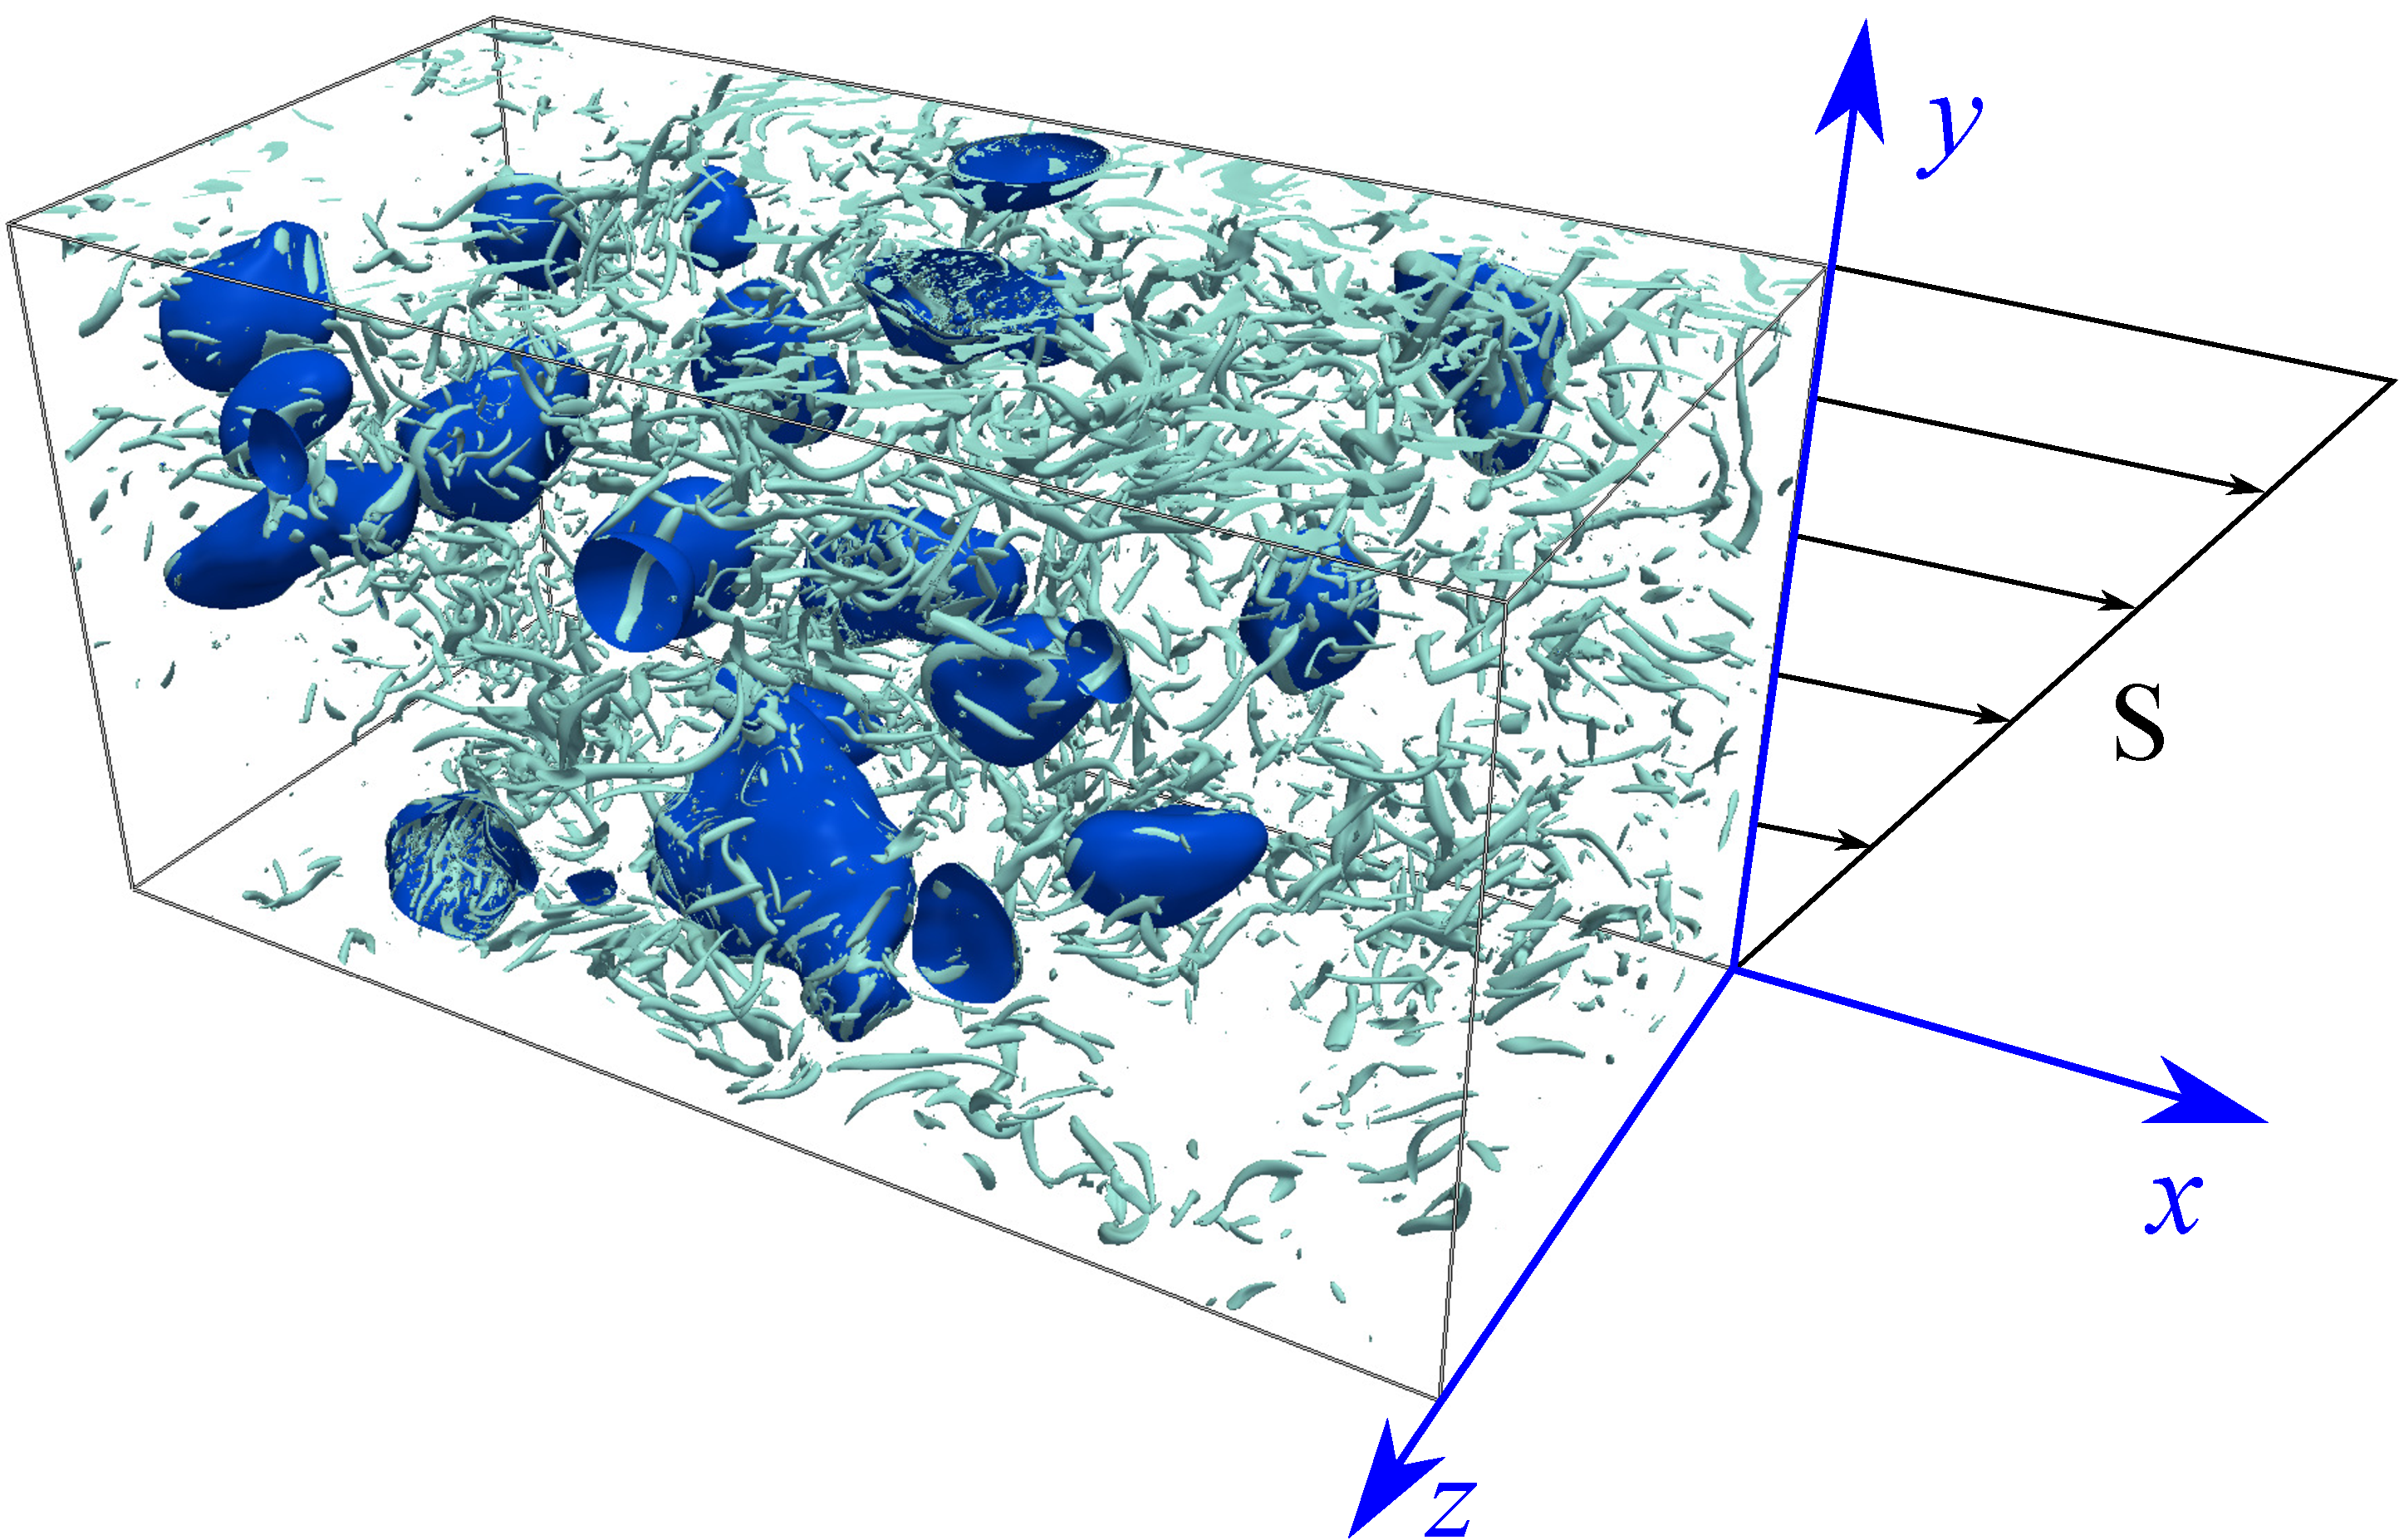
\includegraphics[width=\textwidth,height=0.5\textheight]{../paper_03_toy_model/fig1.eps}\label{fig:sebgcm}}
%%\subfloat[]{\includegraphics[width=\textwidth,height=0.5\textheight]{../paper_03_toy_model/fig10.eps}\label{fig:sebtoy}}
%%
%%\caption{Spectral energy budgets from (a) GCM and (b) toy model
%%simulations.}
%%
%%\label{fig:sebgcmtoy}
%%
%%\end{figure}
%%
%%\begin{itemize}
%%\tightlist
%%\item
%%  where, \(\Pi_{2D} \equiv \Pi_{VVV}\); \(C_{cum}=\) cumulative
%%  conversion function.
%%\item
%%  large-scale forcing in A.P.E. \(\to\) baroclinic instability \(\to\)
%%  conversion to K.E. \(\to\) mesoscale turbulence
%%\end{itemize}
%%\end{frame}
%%
%%\hypertarget{part-2-milestone-experiment}{%
%%\section{Part 2: MILESTONE
%%experiment}\label{part-2-milestone-experiment}}
%%
%%\hypertarget{motivation}{%
%%\subsection{Motivation}\label{motivation}}
%%
%%\begin{frame}{Motivation}
%%\begin{itemize}
%%\tightlist
%%\item
%%  Strongly stratified turbulence regime characterized by
%%  \textbf{horizontal Froude number} and \textbf{buoyancy Reynolds
%%  number}: \[
%%  F_h = \frac{\epsK}{NU^2} \ll 1,\text{ and } \R = ReF_h^2 = \frac{\epsK}{\nu N^2} > 10.
%%  \]
%%\end{itemize}
%%
%%\pause
%%
%%\begin{itemize}
%%\tightlist
%%\item
%%  \textbf{Mixing efficiency} (\(\eta\)) or \textbf{mixing coefficient}
%%  (\(\Gamma\)) are defined as: \[
%%  \eta = \epsP / (\epsK + \epsP),\quad \Gamma = \epsP / \epsK,
%%  \] and widely used to parametrize ocean eddy-diffusivity turbulence
%%  models.
%%\end{itemize}
%%
%%\pause
%%
%%\begin{columns}[T]
%%\begin{column}{0.48\textwidth}
%%\begin{figure}
%%\centering
%%\includegraphics{../imgs/exp-zigzag.png}
%%\caption{Visuals of ``zig-zag instability'' from Billant \&
%%Chomaz(2000)}
%%\end{figure}
%%\end{column}
%%
%%\begin{column}{0.5\textwidth}
%%\begin{block}{Verify results from stratified turbulence theories}
%%\protect\hypertarget{verify-results-from-stratified-turbulence-theories}{}
%%\begin{enumerate}
%%\tightlist
%%\item
%%  \textbf{layered structures} with
%%  \(l_v \sim u/N\)\footnote<.->[frame]{\citet{billant_experimental_2000}}
%%\end{enumerate}
%%
%%~
%%
%%\pause
%%
%%\begin{enumerate}
%%\setcounter{enumi}{1}
%%\tightlist
%%\item
%%  \textbf{forward energy cascade} with
%%  spectrum\footnote<.->[frame]{\citet{Lindborg2006}}
%%  \(E(k) \sim \epsilon^{2/3} k^{-5/3}\), or \(2^{nd}\)-order structure
%%  function scaling\footnote<.->[frame]{\citet{ChoLindborg2001}} as
%%  \(\langle\delta \mathbf{u}. \delta \mathbf{u}\rangle \sim \epsilon^{2/3} r^{2/3}\),
%%  and
%%\end{enumerate}
%%
%%~
%%
%%\pause
%%
%%\begin{enumerate}
%%\setcounter{enumi}{2}
%%\tightlist
%%\item
%%  measure the \textbf{mixing efficiency} in the strongly stratified
%%  regime\footnote<.->[frame]{\citet{maffioli_mixing_2016}}.
%%\end{enumerate}
%%\end{block}
%%\end{column}
%%\end{columns}
%%\end{frame}
%%
%%\hypertarget{experimental-setup}{%
%%\subsection{Experimental Setup}\label{experimental-setup}}
%%
%%\begin{frame}{Experimental Setup}
%%\begin{columns}[T]
%%\begin{column}{0.5\textwidth}
%%\begin{figure}
%%\centering
%%
%%\subfloat[Schematic of the Coriolis platform and mounted instruments
%%(top
%%view)]{\includegraphics[width=\textwidth,height=0.4\textheight]{../paper_05_milestone_issf/Figures/scheme_exp_grid_MILESTONE_Euhit.pdf}\label{fig:scheme-coriolis}}
%%
%%\subfloat[Top view of the
%%setup]{\includegraphics[width=\textwidth,height=0.3\textheight]{../imgs/MILESTONE/GOPR1465.JPG}\label{fig:exp-top}}
%%
%%\caption{Experimental setup}
%%
%%\label{fig:scheme}
%%
%%\end{figure}
%%\end{column}
%%
%%\begin{column}{0.48\textwidth}
%%\begin{block}{Equipment}
%%\protect\hypertarget{equipment}{}
%%\begin{itemize}
%%\tightlist
%%\item
%%  1 \textbf{horizontal} scanning (2D-2C) PIV system
%%\item
%%  1 \textbf{vertical} stereoscopic (2D-3C) PIV system
%%\item
%%  5 conductometric / density \textbf{probes}
%%\item
%%  1 oscillating \textbf{carriage} with 6 cylinders of diameter 0.25 m
%%\item
%%  open-source software for control, calibration, data acquisition etc.
%%\end{itemize}
%%
%%~
%%
%%\centering{%
%%  {%
%%  \movie[
%%    width=7cm,
%%    height=4cm,
%%    showcontrols,
%%    poster,
%%    autostart, loop
%%  ]{}{./videos/moving_carriage.mp4}
%%
%%  Video: Carriage in the Coriolis platform}
%%}
%%\end{block}
%%\end{column}
%%\end{columns}
%%\end{frame}
%%
%%\hypertarget{preliminary-results}{%
%%\subsection{Preliminary results}\label{preliminary-results}}
%%
%%\begin{frame}{Preliminary results: layered
%%structures\footnote<.->[frame]{\citet{ISSF2016}}}
%%\protect\hypertarget{preliminary-results-layered-structures}{}
%%\begin{itemize}
%%\tightlist
%%\item
%%  Vertical length scale\footnote<.->[frame]{\citet{Billant2001}},
%%  \(l_v = u / N\)
%%\end{itemize}
%%
%%\begin{figure}
%%\centerline{
%%\includegraphics[height=0.39\textheight]{../paper_05_milestone_issf/Figures/exp21/vh_400.pdf}
%%\includegraphics[height=0.39\textheight]{../paper_05_milestone_issf/Figures/exp21/vh_655.pdf}
%%\includegraphics[height=0.39\textheight]{../paper_05_milestone_issf/Figures/exp21/vh_890.pdf}}
%%\vspace{0mm}
%%\centerline{
%%\includegraphics[height=0.37\textheight]{../paper_05_milestone_issf/Figures/exp21/vv_890.pdf}
%%\includegraphics[height=0.37\textheight]{../paper_05_milestone_issf/Figures/exp21/vv_655.pdf}
%%\includegraphics[height=0.37\textheight]{../paper_05_milestone_issf/Figures/exp21/vv_400.pdf}
%%}
%%\vspace{-2mm}
%%\caption{Instantaneous horizontal (top, $z=40$~cm) and vertical
%%fields (bottom) for $F_{hc} = 0.1$ and $\mathcal{R}_c=450$.}
%%\label{fig:field}
%%\end{figure}
%%\vspace{-2mm}
%%\end{frame}
%%
%%\begin{frame}{Preliminary results: horizontal structure
%%function\footnote<.->[frame]{\citet{ISSF2016}}}
%%\protect\hypertarget{preliminary-results-horizontal-structure-function}{}
%%\begin{itemize}
%%\tightlist
%%\item
%%  Second-order structure
%%  function\footnote<.->[frame]{\citet{ChoLindborg2001}}
%%  \(S_h \sim \epsilon^{2/3} r^{2/3}\)
%%\end{itemize}
%%
%%\begin{figure}[ht!]
%%\centerline{
%%\includegraphics[height=0.7\textheight]{../paper_05_milestone_issf/Figures/exp28/normalized_S2_exp28.pdf}}
%%\caption{Normalized $S_h$  as a function of
%%$r/M$ for $F_{hc} = 0.1$ and $\mathcal{R}_c=450$.}
%%\label{fig:S2}
%%\end{figure}
%%\end{frame}
%%
%%\begin{frame}{Preliminary results:
%%mixing\footnote<.->[frame]{\citet{ISSF2016}}}
%%\protect\hypertarget{preliminary-results-mixing}{}
%%\begin{itemize}
%%\tightlist
%%\item
%%  \textbf{Mixing
%%  coefficient}\footnote<.->[frame]{\citet{maffioli_mixing_2016}} in
%%  strongly stratified regime \(\Gamma \to 0.2 ?\) and in weakly
%%  stratified regime \(\Gamma \sim F_h^{-2}\).
%%\end{itemize}
%%
%%\begin{figure}[hb!]
%%\centerline{
%%\includegraphics[width=0.45\textwidth]{../_paper_06_milestone/1st/tmp/fig_energy_pot_vs_time}
%%\includegraphics[width=0.55\textwidth]{../_paper_06_milestone/1st/tmp/fig_dt_pot_energy}
%%}
%%\caption{Evolution of potential energy $E_P$ normalized by linear stratification for
%%experiment M17-21 (left) and normalized mixing coefficient $\eps_P /
%%(3\times10^{-3} {U_c}^3/D_c)$ for some MILESTONE 17 experiments (right).}%
%%\label{fig:dt:pot:energy}
%%\end{figure}
%%\end{frame}
%%
%%\hypertarget{part-3-reproducible-open-science-through-open-source}{%
%%\section{Part 3: Reproducible open science through open
%%source}\label{part-3-reproducible-open-science-through-open-source}}
%%
%%\hypertarget{open-science}{%
%%\subsection{Open science}\label{open-science}}
%%
%%\begin{frame}{Open science}
%%\begin{columns}[T]
%%\begin{column}{0.48\textwidth}
%%\includegraphics[width=0.9\textwidth,height=\textheight]{../imgs/open_science.pdf}
%%\end{column}
%%
%%\begin{column}{0.6\textwidth}
%%\begin{block}{Path to reproducible research}
%%\protect\hypertarget{path-to-reproducible-research}{}
%%\pause
%%
%%\begin{itemize}
%%\tightlist
%%\item
%%  Accessible knowledge: {\color{violet}{open access}}
%%\end{itemize}
%%
%%\pause
%%
%%\begin{itemize}
%%\item
%%  Accessible implementation:
%%  {\color{Cerulean}{{license + open source code}}}
%%\item
%%  Reliability: {\color{Cerulean}{documentation, continuous integration}}
%%\end{itemize}
%%
%%\pause
%%
%%\begin{itemize}
%%\item
%%  Open data: {\color{SeaGreen}{citable datasets}}
%%\item
%%  Tracking workflow: {\color{SeaGreen}{version control}}
%%\end{itemize}
%%
%%\pause
%%
%%\begin{itemize}
%%\tightlist
%%\item
%%  Publish: {\color{DarkGoldenrod}{manuscript + data + code + workflow}}
%%\end{itemize}
%%
%%\pause
%%\end{block}
%%
%%\begin{block}{Arguments for open source}
%%\protect\hypertarget{arguments-for-open-source}{}
%%\begin{itemize}
%%\item
%%  Reproducibility
%%\item
%%  Peer review for both manuscript and code
%%\item
%%  Interoperable and sustainable
%%\item
%%  Public money, public code\footnote<.->[frame]{https://publiccode.eu}
%%\end{itemize}
%%
%%\pause
%%\end{block}
%%
%%\begin{block}{Arguments against open source}
%%\protect\hypertarget{arguments-against-open-source}{}
%%\begin{itemize}
%%\item
%%  Comparative advantage
%%\item
%%  Lack of support
%%\item
%%  Curb industrial usage
%%\item
%%  Lack of documentation / not near production quality
%%\end{itemize}
%%\end{block}
%%\end{column}
%%\end{columns}
%%\end{frame}
%%
%%\begin{frame}{Python programming language}
%%\protect\hypertarget{python-programming-language}{}
%%\begin{itemize}
%%\item
%%  One of the most popular
%%  languages\footnote<.->[frame]{Stack Overflow, GitHub, TIOBE index, IEEE spectrum}
%%  in the world
%%\item
%%  General purpose
%%\item
%%  Thriving scientific community
%%\end{itemize}
%%
%%\begin{columns}[T]
%%\begin{column}{0.5\textwidth}
%%\includegraphics[width=0.9\textwidth,height=\textheight]{../imgs/python-sci-ecosystem.png}
%%\end{column}
%%
%%\begin{column}{0.48\textwidth}
%%\includegraphics[width=0.9\textwidth,height=\textheight]{../imgs/python-popularity.png}
%%\end{column}
%%\end{columns}
%%\end{frame}
%%
%%\begin{frame}{Why Python in sciences?}
%%\protect\hypertarget{why-python-in-sciences}{}
%%\begin{greencolorbox}[Advantages]\label{advantages}
%%
%%\begin{itemize}
%%\item
%%  Simple learning curve
%%\item
%%  Rapid prototyping
%%\item
%%  Expressive to communicate ideas
%%\item
%%  Extensible
%%\item
%%  Batteries included: powerful standard libraries
%%\end{itemize}
%%
%%\end{greencolorbox}
%%
%%\begin{bluecolorbox}[Issues and solutions]\label{issues-and-solutions}
%%
%%\begin{itemize}
%%\tightlist
%%\item
%%  CPU bounded performance
%%
%%  \begin{itemize}
%%  \tightlist
%%  \item
%%    native (C, C++ or Fortran), compiled (AOT or JIT)
%%    \textbf{extensions} for hotspots
%%  \end{itemize}
%%\item
%%  Concurrent, but no parallel threading
%%
%%  \begin{itemize}
%%  \tightlist
%%  \item
%%    use \textbf{multiprocessing} / \textbf{MPI}
%%  \end{itemize}
%%\end{itemize}
%%
%%\end{bluecolorbox}
%%\end{frame}
%%
%%\hypertarget{fluiddyn-project}{%
%%\subsection{FluidDyn project}\label{fluiddyn-project}}
%%
%%\begin{frame}[fragile]{FluidDyn project}
%%\begin{columns}[T]
%%\begin{column}{0.45\textwidth}
%%\begin{figure}
%%\centering
%%\includegraphics[width=0.9\textwidth,height=\textheight]{../imgs/logo-fluiddyn.jpg}
%%\caption{Project to foster open-science and open-source in fluid
%%mechanics}
%%\end{figure}
%%
%%\pause
%%
%%\begin{itemize}
%%\item
%%  {\alert<+->{\texttt{fluiddyn}}}: base
%%  package\footnote<.->[frame]{\citet{fluiddyn}}
%%\item
%%  {\alert<+->{\texttt{fluidfft}}}: API for Fast Fourier Transforms
%%\item
%%  {\alert<+->{\texttt{fluidsim}}}: CFD framework
%%\end{itemize}
%%
%%\onslide<+->
%%
%%\begin{itemize}
%%\item
%%  \texttt{fluidimage}: asynchronously parallelized image processing,
%%  including PIV
%%\item
%%  \texttt{fluidlab}: laboratory experiments
%%\item
%%  \texttt{transonic}: front-end for generating Python extensions
%%\end{itemize}
%%\end{column}
%%
%%\begin{column}{0.48\textwidth}
%%\begin{figure}
%%\centering
%%\includegraphics[width=0.9\textwidth,height=\textheight]{../imgs/dependency.pdf}
%%\caption{Standing on the shoulders of giants}
%%\end{figure}
%%\end{column}
%%\end{columns}
%%\end{frame}
%%
%%\begin{frame}[fragile]{Package
%%\texttt{fluidfft}\footnote<.->[frame]{\citet{fluidfft}}}
%%\protect\hypertarget{package-fluidfft}{}
%%\begin{columns}[T]
%%\begin{column}{0.4\textwidth}
%%\begin{itemize}
%%\item
%%  FFT libraries: \texttt{FFTW}, \texttt{P3DFFT}, \texttt{PFFT},
%%  \texttt{cuFFT} interfaced using \texttt{C++} and \texttt{Cython}
%%\item
%%  Pseudospectral ``operator'' classes with \texttt{Pythran} methods
%%\end{itemize}
%%\end{column}
%%
%%\begin{column}{0.48\textwidth}
%%\begin{Shaded}
%%\begin{Highlighting}[]
%%\CommentTok{\# An example for calculating gradient}
%%\ImportTok{from}\NormalTok{ fluidfft.fft2d.operators }\ImportTok{import}\NormalTok{ OperatorsPseudoSpectral2D}
%%\ImportTok{from}\NormalTok{ numpy }\ImportTok{import}\NormalTok{ sin, pi}
%%
%%\NormalTok{oper }\OperatorTok{=}\NormalTok{ OperatorsPseudoSpectral2D(}
%%\NormalTok{  nx}\OperatorTok{=}\DecValTok{100}\NormalTok{, ny}\OperatorTok{=}\DecValTok{100}\NormalTok{, lx}\OperatorTok{=}\DecValTok{2}\OperatorTok{*}\NormalTok{pi, ly}\OperatorTok{=}\DecValTok{2}\OperatorTok{*}\NormalTok{pi, fft}\OperatorTok{=}\StringTok{"fft2d.with\_fftw2d"}
%%\NormalTok{)}
%%\NormalTok{u }\OperatorTok{=}\NormalTok{ sin(oper.XX }\OperatorTok{+}\NormalTok{ oper.YY)}
%%\NormalTok{u\_fft }\OperatorTok{=}\NormalTok{ oper.fft(u)}
%%\NormalTok{px\_u\_fft, py\_u\_fft }\OperatorTok{=}\NormalTok{ oper.gradfft\_from\_fft(u\_fft)}
%%\end{Highlighting}
%%\end{Shaded}
%%\end{column}
%%\end{columns}
%%
%%\begin{figure}
%%\centering
%%\includegraphics[width=\textwidth,height=0.5\textheight]{../paper_01_fluidfft/Pyfig/fig_classes.pdf}
%%\caption{Class hierarchy of {\color{Salmon}{\emph{sequential}}},
%%{\color{magenta}{\emph{CUDA}}}, {\color{SeaGreen}{\emph{MPI}}} FFT
%%libraries}
%%\end{figure}
%%\end{frame}
%%
%%\begin{frame}{Performance of
%%\texttt{fluidfft}\footnote<.->[frame]{\citet{fluidfft}}: scaling}
%%\protect\hypertarget{performance-of-fluidfft-scaling}{}
%%\begin{figure}
%%\centering
%%\includegraphics[width=1.3\textwidth,height=\textheight]{../paper_01_fluidfft/tmp/fig_beskow_1152x1152x1152.pdf}
%%\caption{Strong scaling of 3D FFT upto 10000 cores}
%%\end{figure}
%%\end{frame}
%%
%%\begin{frame}[fragile]{Performance of
%%\texttt{fluidfft}\footnote<.->[frame]{\citet{fluidfft}}:
%%microbenchmarks}
%%\protect\hypertarget{performance-of-fluidfft-microbenchmarks}{}
%%\begin{itemize}
%%\tightlist
%%\item
%%  \texttt{Pythran} extensions comparable compiled native languages
%%\item
%%  Memory allocation is expensive: \textbf{in-place} better than
%%  \textbf{out-of-place}
%%\end{itemize}
%%
%%\begin{figure}
%%\centering
%%\includegraphics[width=1\textwidth,height=\textheight]{../paper_01_fluidfft/tmp/fig_microbench.pdf}
%%\caption{Microbenchmarks of projection function}
%%\end{figure}
%%\end{frame}
%%
%%\begin{frame}[fragile]{Package
%%\texttt{fluidsim}\footnote<.->[frame]{\citet{fluidsim}}}
%%\protect\hypertarget{package-fluidsim}{}
%%\begin{columns}[T]
%%\begin{column}{0.4\textwidth}
%%\begin{itemize}
%%\item
%%  Extensible, object-oriented CFD framework
%%\item
%%  On-the-fly post-processing
%%\item
%%  Code reuse: \texttt{numpy}, \texttt{fluiddyn}, \texttt{fluidfft} etc.
%%\end{itemize}
%%\end{column}
%%
%%\begin{column}{0.48\textwidth}
%%\begin{Shaded}
%%\begin{Highlighting}[]
%%\CommentTok{\# An example for running 3D Navier Stokes solver}
%%\ImportTok{from}\NormalTok{ fluidsim.solvers.ns3d.solver }\ImportTok{import}\NormalTok{ Simul}
%%
%%\NormalTok{params }\OperatorTok{=}\NormalTok{ Simul.create\_default\_params()}
%%\CommentTok{\# Modify parameters as needed}
%%\NormalTok{sim }\OperatorTok{=}\NormalTok{ Simul(params)}
%%\NormalTok{sim.time\_stepping.start()}
%%\end{Highlighting}
%%\end{Shaded}
%%\end{column}
%%\end{columns}
%%
%%\pause
%%
%%\begin{figure}
%%\centering
%%\includegraphics[width=\textwidth,height=0.55\textheight]{../paper_02_fluidsim/tmp/fig_profile3d.pdf}
%%\caption{Profiling \texttt{fluidsim.solvers.ns3d.solver}}
%%\end{figure}
%%\end{frame}
%%
%%\begin{frame}[fragile]{Performance of
%%\texttt{fluidsim}\footnote<.->[frame]{\citet{fluidsim}}: profiling}
%%\protect\hypertarget{performance-of-fluidsim-profiling}{}
%%\begin{figure}
%%\centering
%%\includegraphics[width=1.3\textwidth,height=\textheight]{../paper_02_fluidsim/tmp/fig_compare_with_ns3d.pdf}
%%\caption{Comparison of {\color{blue}{Fortran code NS3D}} with
%%{\color{DarkGoldenrod}{\texttt{fluidsim.solvers.ns3d.solver}}}}
%%\end{figure}
%%\end{frame}
%%
%%\begin{frame}[fragile]{Performance of
%%\texttt{fluidsim}\footnote<.->[frame]{\citet{fluidsim}}: scaling}
%%\protect\hypertarget{performance-of-fluidsim-scaling}{}
%%\begin{figure}
%%\centering
%%\includegraphics[width=1.3\textwidth,height=\textheight]{../paper_02_fluidsim/tmp/fig_bench_strong3d.pdf}
%%\caption{Strong scaling for \texttt{fluidsim.solvers.ns3d.solver} using
%%{\color{MidnightBlue}{FFTW-MPI}} and {\color{BurntOrange}{P3DFFT}} via
%%\texttt{fluidfft}}
%%\end{figure}
%%\end{frame}
%%
%%\hypertarget{concluding-remarks}{%
%%\section{Concluding remarks}\label{concluding-remarks}}
%%
%%\begin{frame}{Concluding remarks}
%%\protect\hypertarget{concluding-remarks-1}{}
%%\begin{block}{Part 1}
%%\protect\hypertarget{part-1}{}
%%\begin{itemize}
%%\item
%%  Scaling relations for \textbf{shock} dominated turbulence
%%\item
%%  Developed a toy-model which exhibits \textbf{forward cascade} in
%%  ``mesoscales'' with a \(k^{-5/3}\) spectrum
%%\end{itemize}
%%
%%\pause
%%\end{block}
%%
%%\begin{block}{Part 2}
%%\protect\hypertarget{part-2}{}
%%\begin{itemize}
%%\item
%%  Verified \textbf{vertical length scale} \(l_v \sim u/N\) and
%%  \textbf{forward cascade} \(S_h \sim \epsilon^{2/3}r^{2/3}\)
%%\item
%%  Mixing coefficient (\(\Gamma\)) estimates requires further
%%  investigations
%%\end{itemize}
%%
%%\pause
%%\end{block}
%%
%%\begin{block}{Part 3}
%%\protect\hypertarget{part-3}{}
%%\begin{itemize}
%%\item
%%  Python as primary language for building research software
%%\item
%%  Good \textbf{performance} by optimising bottlenecks
%%\end{itemize}
%%\end{block}
%%\end{frame}
%%
